\chapter{Esperimenti di simulazione}\label{chp:esperimenti-simulazione}
In accordo agli obiettivi dello studio, per la progettazione degli esperimenti di simulazione, è stata considerata unicamente l'analisi dello stato transiente del sistema. Infatti, perderebbe di significato considerare lo stato stazionario per determinare il numero minimo di serventi necessari affinché vengano soddisfatti i QoS descritti nel capitolo \ref{chp:obiettivi}. Questo perché in una giornata lavorativa, assunta pari ad otto ore, il sistema non riesce a raggiungere lo stato stazionario prima che si verifichi la condizione di scarico (\textit{"close the door"}) ed inoltre rimane forte l'influenza delle condizioni iniziali.

\section{Progetto degli esperimenti}
Per realizzare l'analisi transiente del sistema è stata adottata la tecnica \textit{replication} utilizzando i seguenti parametri:
\begin{itemize}
\item \texttt{TERM\_INIT\_SEED = 9}, settato unicamente a inizio simulazione al fine di rendere le repliche tra loro indipendenti 
\item \texttt{ENSEMBLE\_SIZE = 300}, al fine di perdere la dipendenza dal seme iniziale pur mantenendo la variabilità naturale del fenomeno osservato.
\item \texttt{START = 0} e \texttt{STOP = 480} come descritto in sezione \ref{sec:modello-computazionale-clock}.
\end{itemize}

Inoltre:
\begin{itemize}
\item È stato utilizzato il programma \texttt{estimate} per il calcolo delle realizzazioni degli intervalli di confidenza.
\item È stato utilizzato il programma \texttt{uvs} per il calcolo di media, deviazione standard, massimo e minimo.
\end{itemize}

\subsection*{Numero minimo di sportelli}
Per individuare il numero minimo $M^*$ di sportelli da mantenere operativi in una giornata lavorativa, al fine di soddisfare i QoS (cap. \ref{chp:obiettivi}), un primo esperimento condotto è stato quello di analizzare l'attesa media di ciascun flusso d'arrivo al variare di $M$.

A tal proposito, è stato simulato il sistema per un'intera giornata di lavoro, assumendo che i clienti iniziassero ad arrivare all'ufficio postale \textbf{solo} successivamente all'apertura (sistema inizialmente scarico).

\subsection*{Attesa nell'arco della giornata a partire dal sistema scarico}
Una volta individuato il valore $M^*$, è stata studiata l'evoluzione dell'attesa media per ciascun flusso d'arrivo all'avanzare del tempo di simulazione.

Per realizzare quest'esperimento, la simulazione è stata arrestata ogni:
\begin{equation}
\begin{array}{l l l l l l}
45\ min, & 45 + 2\ min, & 45 + 2^2\ min, & \dots, & 45 + 2^8\ min, & 480\ min
\end{array}
\end{equation}
per le seguenti motivazioni:
\begin{itemize}
\item È stato scelto di partire da $45\ min$ per consentire la formazione delle code (poiché il sistema parte da scarico).
\item La crescita esponenziale per potenze di 2 successive permette di avere una visione a grana fine negli intervalli iniziali, dove per via della carica del sistema, è più probabile vi sia una maggiore variabilità dell'andamento del tempo di coda. 
\end{itemize}

\subsection*{Attesa nell'arco della giornata a partire da condizioni iniziali non nulle}
Per enfatizzare l'impatto delle condizioni iniziali sulle prestazioni del sistema, è stato replicato l'esperimento precedente assumendo che all'apertura dell'ufficio postale vi fossero già dei clienti in attesa di essere serviti.

Per ciascuna tipologia di flusso, il numero iniziale di clienti è stato impostato pari alla parte intera superiore della rispettiva popolazione media calcolata a partire da condizioni iniziali nulle, ovvero:
\begin{equation}
Customers_i(0) = \lceil\ \bar{l}_i\ \rceil
\end{equation}
in riferimento alla definizione nella \ref{eqn:modello-specifiche-2}.
	
\section{Esecuzione degli esperimenti ed analisi degli output}

\begin{figure}[ht]
\centering
\begin{subfigure}[b]{0.475\textwidth}
\centering
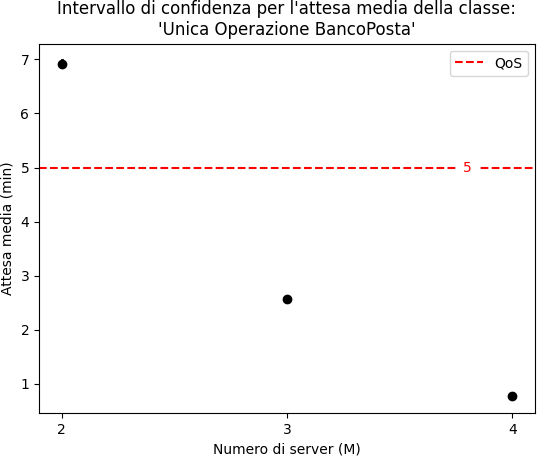
\includegraphics[width=\textwidth]{plots/d0-trans}
\caption{Tempo medio d'attesa per ticket di tipo 0}    
\label{fig:esperimenti-simulazione-a}
\end{subfigure}
\hfill    
\begin{subfigure}[b]{0.475\textwidth}  
\centering 
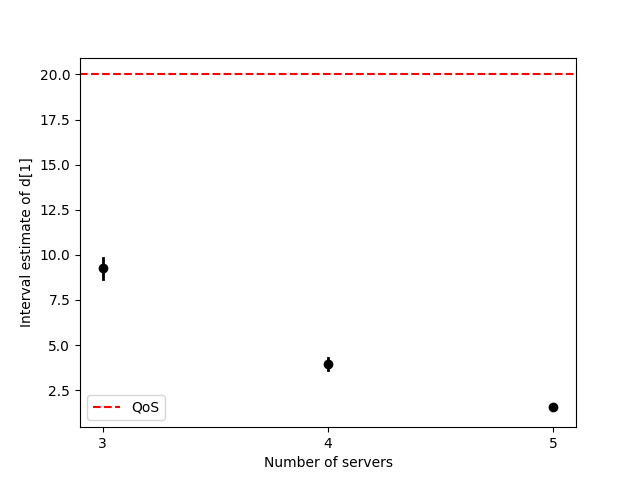
\includegraphics[width=\textwidth]{plots/d1-trans}
\caption{Tempo medio d'attesa per ticket di tipo 1}    
\label{fig:esperimenti-simulazione-b}
\end{subfigure}


\vskip\baselineskip

\begin{subfigure}[b]{0.475\textwidth}   
\centering 
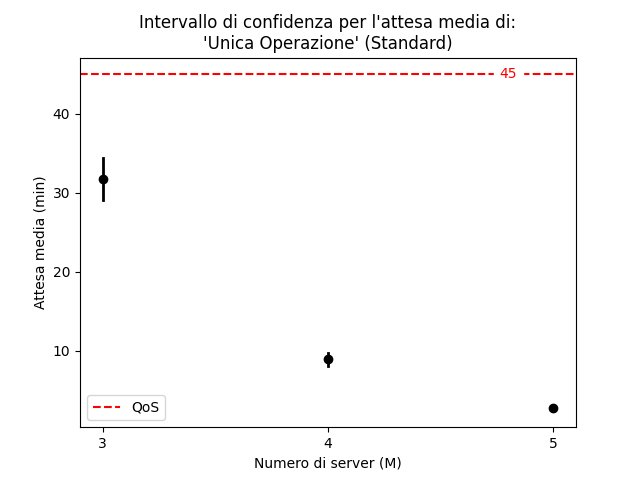
\includegraphics[width=\textwidth]{plots/d2-trans}
\caption{Tempo medio d'attesa per ticket di tipo 2}    
\label{fig:esperimenti-simulazione-c}
\end{subfigure}
\hfill
\begin{subfigure}[b]{0.475\textwidth}   
\centering 
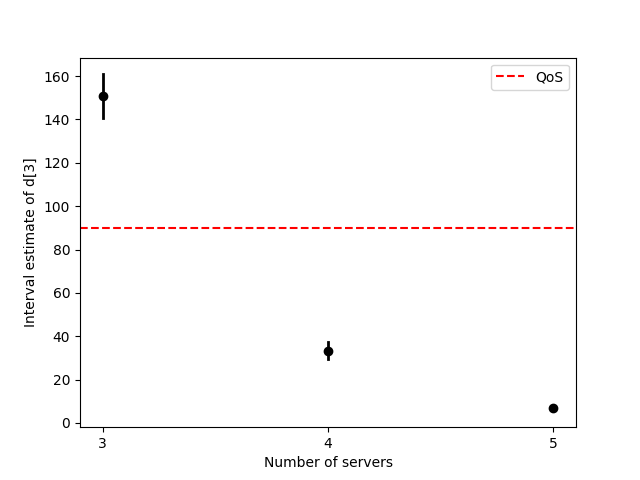
\includegraphics[width=\textwidth]{plots/d3-trans}
\caption{Tempo medio d'attesa per ticket di tipo 3}    
\label{fig:esperimenti-simulazione-d}
\end{subfigure}

\vskip\baselineskip

\begin{subfigure}[b]{0.475\textwidth}   
\centering 
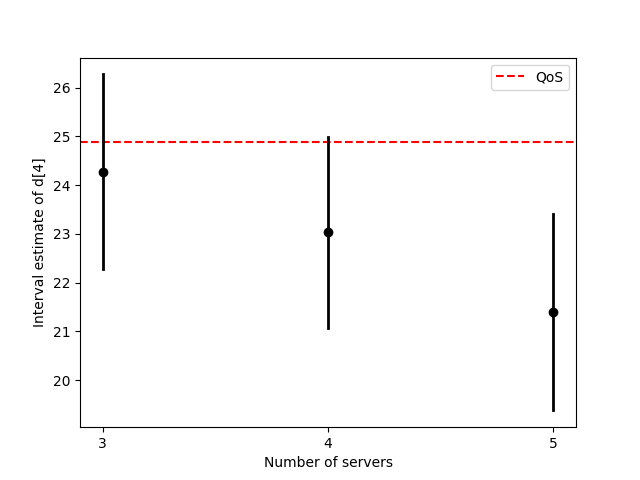
\includegraphics[width=\textwidth]{plots/d4-trans}
\caption{Tempo medio d'attesa per ticket di tipo 4}    
\label{fig:esperimenti-simulazione-e}
\end{subfigure}
\hfill
\begin{subfigure}[b]{0.475\textwidth}   
\centering 
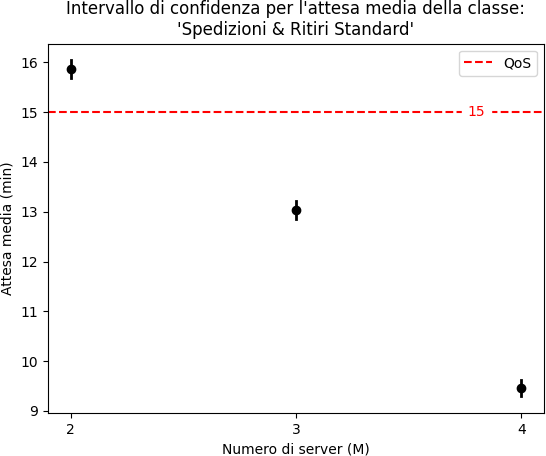
\includegraphics[width=\textwidth]{plots/d5-trans}
\caption{Tempo medio d'attesa per ticket di tipo 5}    
\label{fig:esperimenti-simulazione-f}
\end{subfigure}
\caption{Tempi medi d'attesa al variare di $M$ (id dei ticket in tabella \ref{table:modello-specifiche-1})}
\label{fig:esperimenti-simulazione}
\end{figure}


